\chapter{Tests and Results}\label{chap:test}
This chapter presents the results of the tests conducted and the module validation.

\section{Algorithm Analysis and Tests}\label{sec:alg_anal}

\subsection{Data Metrics}\label{sec:bench}
The project aims to provide fast and efficient MVMs for matrices stored in PCM memory up to 2 layers of $512\;\times\;512$ with $8$ bit weights and $8$ bit integer inputs.
For this reason, experiments consider matrix dimensions up to $512\;\times\;512$.
All tests were executed after a clean start-up to minimise noise given by other applications for context switching and synchronization inside the CPU scheduler.
The results come from batch runs of 100 pseudo-random matrices sequentially computed with different algorithms and different setups.
This approach reduces the noise given by comparing different matrix configurations and focuses on the performance of the algorithm itself.
We conducted tests using two profiles, one with optimisation switched on and the other off, to see how compiler optimisations affect the results.

\subsubsection{Performances Data}\label{sec:Data_Perf}
The main metric used to evaluate the performance of the algorithms is the time to complete a single MVM computed with the aid of the $std::high_resolution_clock$.
\begin{figure}[!htb]
\begin{minipage}{1\textwidth}
    {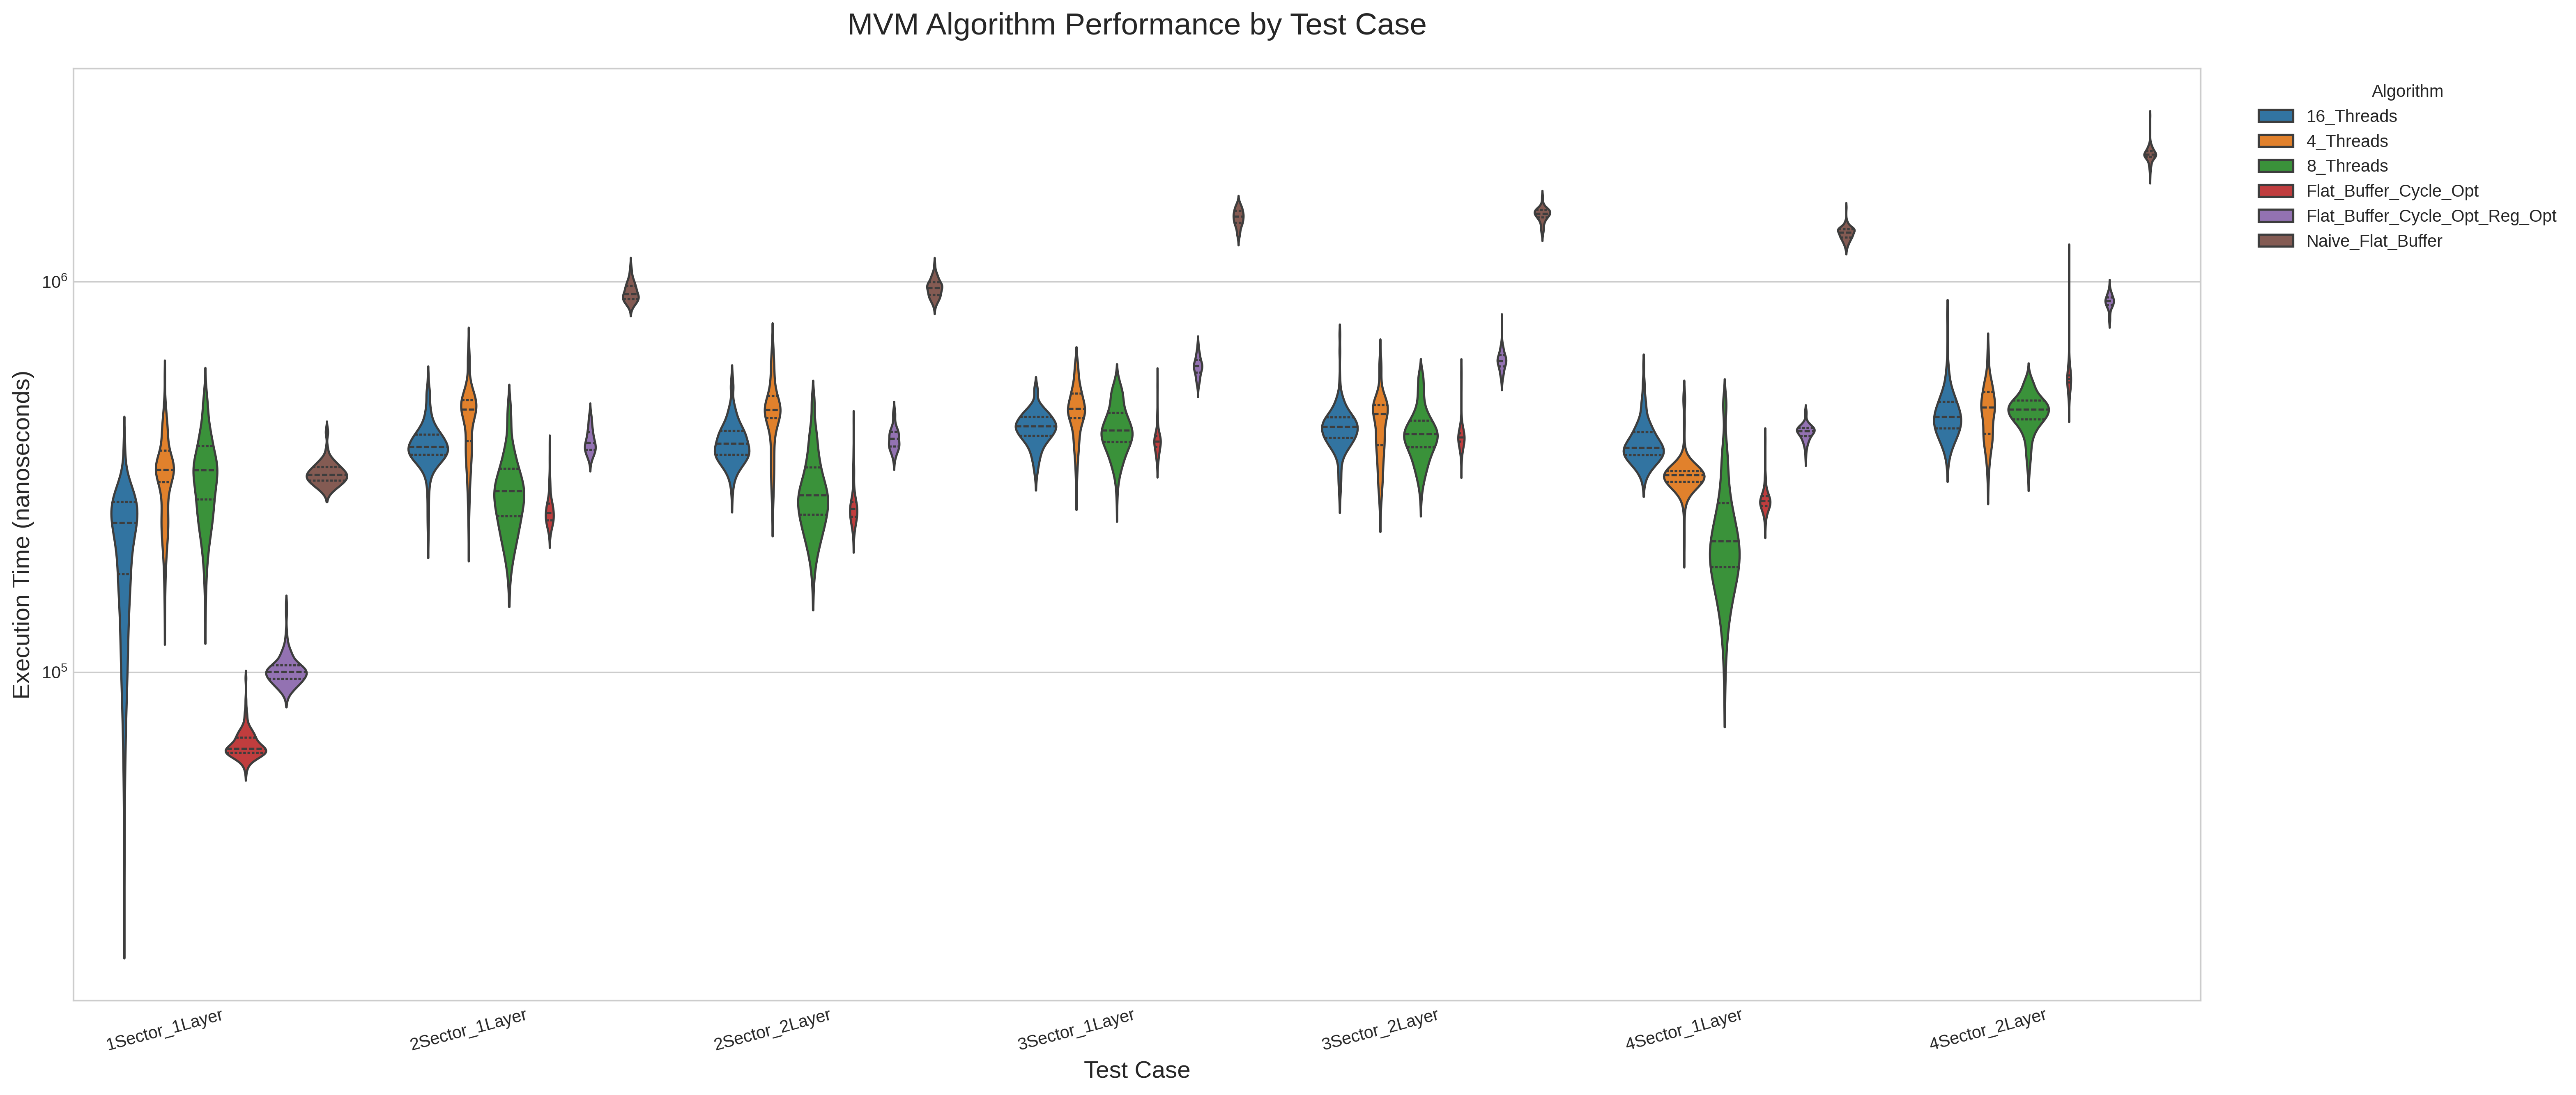
\includegraphics[width=\textwidth]{Figures/mvm_benchmark_violin_plot (1).png}
    \label{fig:no_opt_plot}}
\end{minipage}
\hfill
\begin{minipage}{1\textwidth}
    {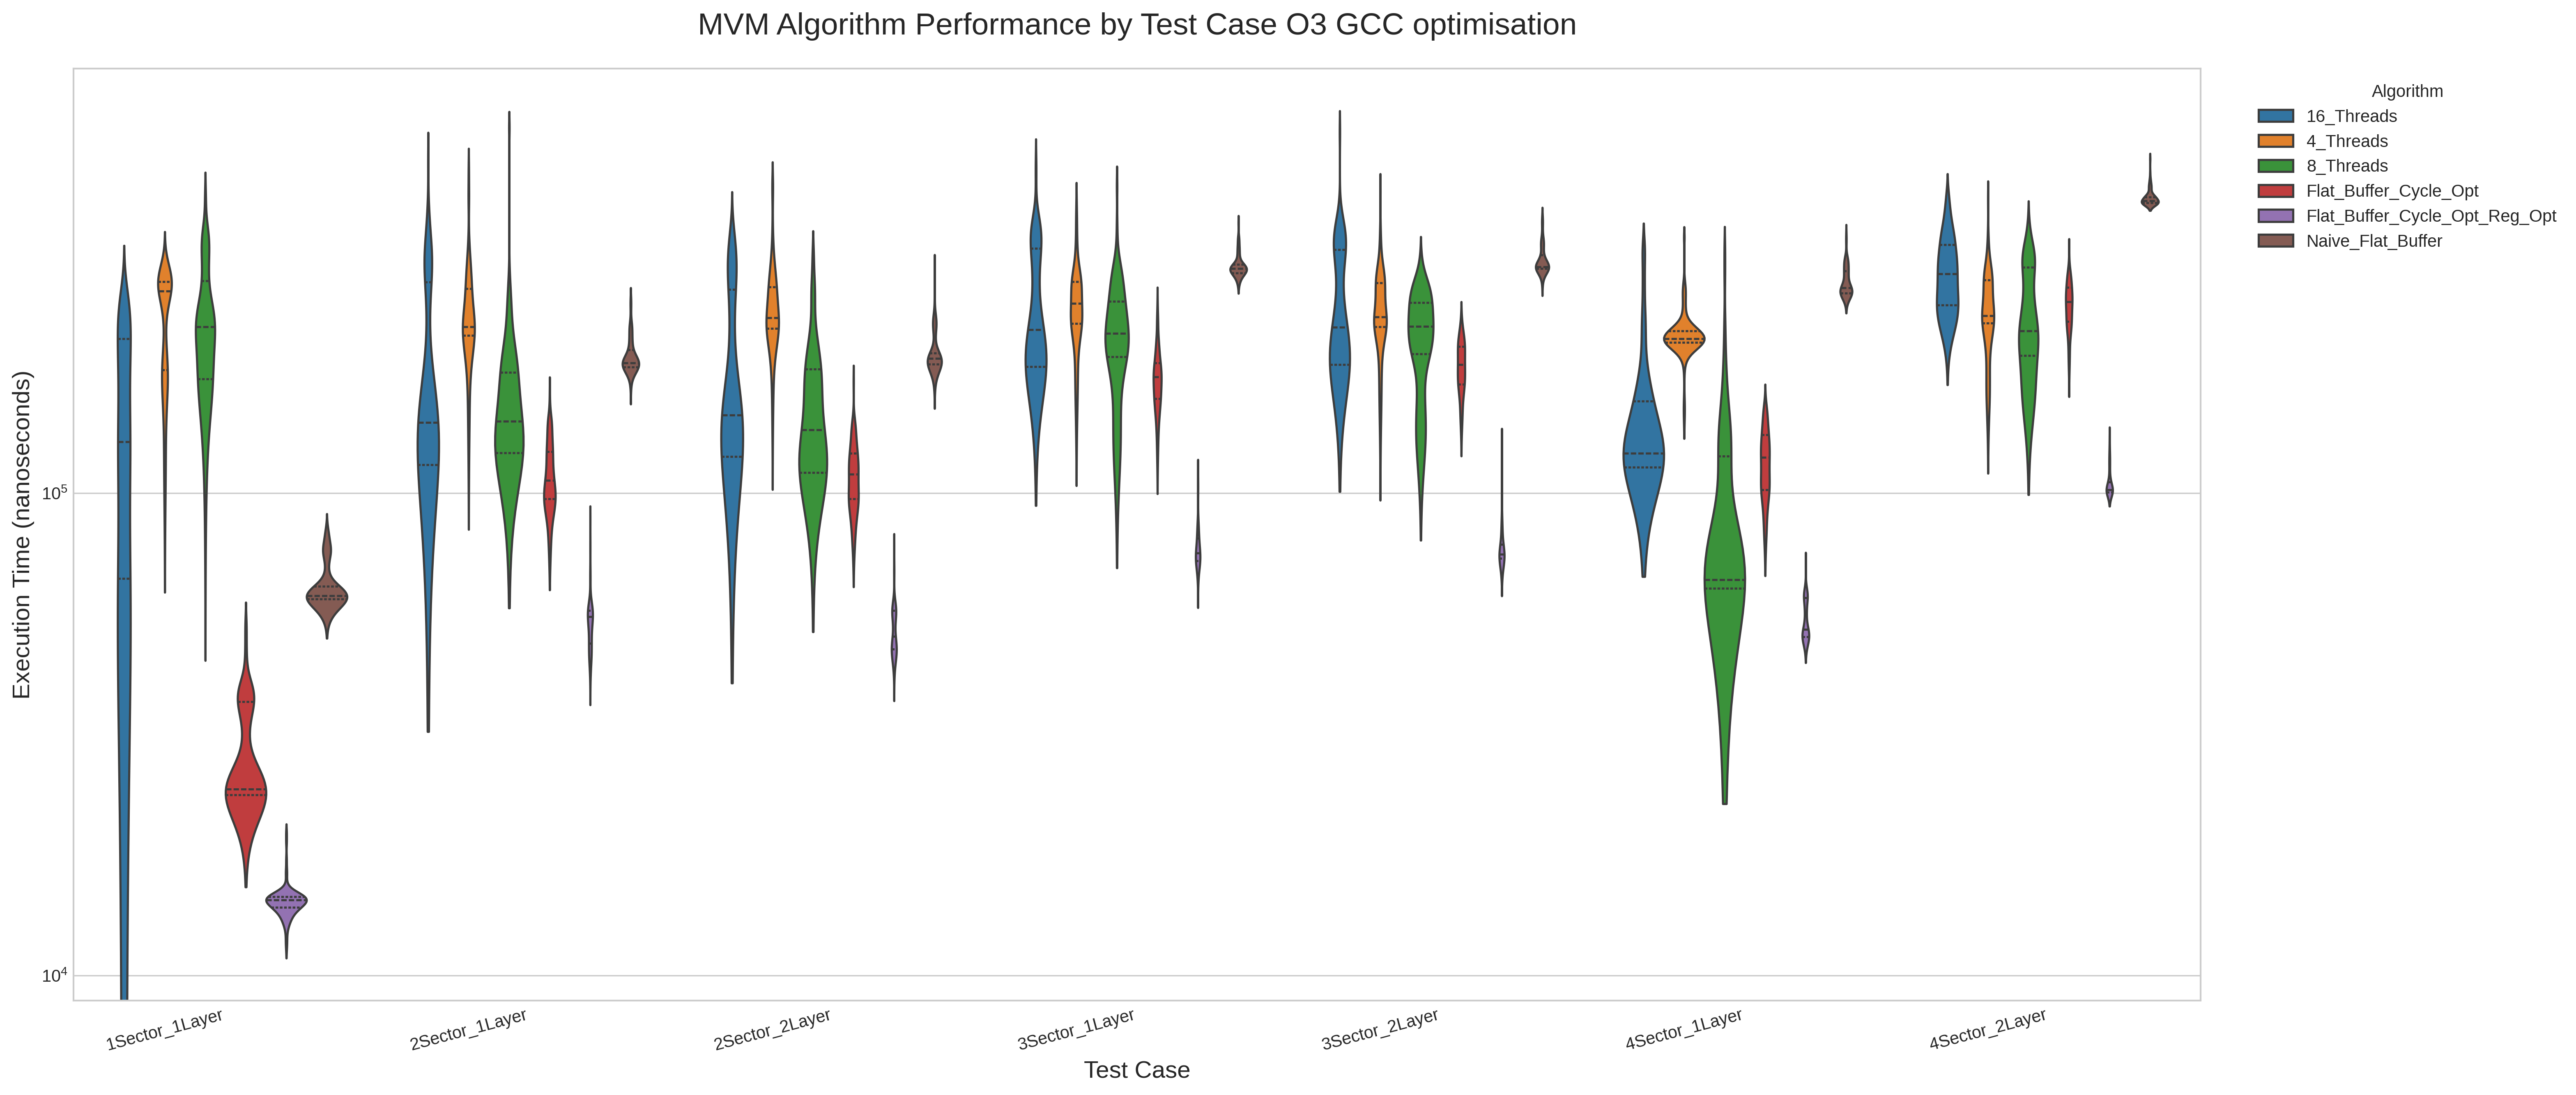
\includegraphics[width=\textwidth]{Figures/mvm_benchmark_violin_plot_opt.png}
    \label{fig:opt_plot}}
\end{minipage}
\caption{\\ Violin plots of the results with and without optimisation. \label{fig:plots}}
\end{figure}

\begin{table}[htbp]
\centering
\caption{Cachegrind Performance Counters for Optimised MVM Algorithms (-O3)}
\label{tab:cachegrind_o3_revised}
\sisetup{group-separator={,}}

\resizebox{\textwidth}{!}{
\begin{tabular}{
  l 
  S[table-format=7.0]
  S[table-format=7.0]
  S[table-format=4.0]
  S[table-format=6.0]
  S[table-format=7.0]
  S[table-format=4.0]
}
\toprule
\textbf{Algorithm} &
{\begin{tabular}[c]{@{}c@{}}\textbf{Instructions}\\(\textbf{Ir})\end{tabular}} &
{\begin{tabular}[c]{@{}c@{}}\textbf{Data Reads}\\(\textbf{Dr})\end{tabular}} &
{\begin{tabular}[c]{@{}c@{}}\textbf{L1 Read}\\\textbf{Misses}\end{tabular}} &
{\begin{tabular}[c]{@{}c@{}}\textbf{Data Writes}\\(\textbf{Dw})\end{tabular}} &
{\begin{tabular}[c]{@{}c@{}}\textbf{Branches}\\(\textbf{Bc})\end{tabular}} &
{\begin{tabular}[c]{@{}c@{}}\textbf{Branch}\\\textbf{Misses}\end{tabular}} \\
\midrule
Naive     & 7343702 & 1311265 & 8270 & 262154 & 1049093 & 534   \\
Optimise  & 1814663 & 66586   & 8340 & 1027   & 33809   & 1077  \\
4-Thread  & 1814672 & 66580   & 8346 & 1024   & 33804   & 1071  \\
8-Thread  & 1808472 & 65544   & 8211 & 0      & 33792   & 1050  \\
16-Thread & 1807632 & 65552   & 8232 & 0      & 33808   & 1066  \\
\bottomrule
\end{tabular}
}
\end{table}

\begin{table}[htbp]
\centering
\caption{Cachegrind Performance Counters for Unoptimised MVM Algorithms (-O0)}
\label{tab:cachegrind_o0}
\sisetup{group-separator={,}}

\resizebox{\textwidth}{!}{
\begin{tabular}{
  l 
  S[table-format=7.0]
  S[table-format=7.0]
  S[table-format=4.0]
  S[table-format=6.0]
  S[table-format=7.0]
  S[table-format=4.0]
}
\toprule
\textbf{Algorithm} &
{\begin{tabular}[c]{@{}c@{}}\textbf{Instructions}\\(\textbf{Ir})\end{tabular}} &
{\begin{tabular}[c]{@{}c@{}}\textbf{Data Reads}\\(\textbf{Dr})\end{tabular}} &
{\begin{tabular}[c]{@{}c@{}}\textbf{L1 Read}\\\textbf{Misses}\end{tabular}} &
{\begin{tabular}[c]{@{}c@{}}\textbf{Data Writes}\\(\textbf{Dw})\end{tabular}} &
{\begin{tabular}[c]{@{}c@{}}\textbf{Branches}\\(\textbf{Bc})\end{tabular}} &
{\begin{tabular}[c]{@{}c@{}}\textbf{Branch}\\\textbf{Misses}\end{tabular}} \\
\midrule
Naive     & 33820273  & 14681640  & 8260 & 1311250  & 1049609 & 555 \\
Optimised & 8419725   & 4730004   & 8335 & 3126     & 526361  & 1070 \\
4-Thread  & 8419688   & 4729980   & 8338 & 3140     & 526356  & 1064 \\
8-Thread  & 8410232   & 4725784   & 8200 & 5168     & 526344  & 1055 \\
16-Thread & 8411440   & 4726864   & 8214 & 5248     & 526352  & 1061 \\
\bottomrule
\end{tabular}
}
\end{table}


\subsection{Performance Analysis}\label{sec:data_anal}
The benchmark results demonstrate that the optimised implementation achieves approximately $4\times$ speedup over the naive approach when compiled with the O3 flag. 
This performance gain derives from the combined effect of algorithmic improvements and compiler optimisations.\\
The following sections analyze each optimisation technique individually to understand each contribution.

\subsubsection{Impact of Compiler optimisations}\label{sec:compiler_impact}
Figure \ref{fig:plots} shows the execution time distribution for different algorithm variants compiled with both O0 and O3 flags. 
The compiler optimisation level has a great impact on all implementations, with O3 producing on average $2\times$ faster code across all tested algorithms.
Using O3, even the naive implementation benefits from compiler optimisations, though it remains the slowest one. 
The only exception takes place with very small matrices, where the multithreaded overhead exceeds the benefit of parallelization.
Notably, compiler optimisation interacts differently with our algorithmic improvements depending on the optimisation level. 
Under O0, the 8-thread implementation outperforms the optimised single-threaded version, as our hand-coded optimisations cannot compensate for the lack of compiler support. 
However, under O3, the single-threaded optimised version becomes the fastest option, as the compiler can make good use of the optimisations we implemented through improved data structures and memory access patterns.

\subsubsection{Cache Behavior}\label{sec:cache_beh}
Tables \ref{tab:cachegrind_o3_revised} and \ref{tab:cachegrind_o0} present detailed performance counters collected using Valgrind's Cachegrind tool.
These metrics provide more data on how each algorithm interacts with the CPU cache hierarchy.
Starting with the instruction counts (Ir), we observe a $4\times$ reduction in instructions executed. This outcome aligns with the overall memory access reductions seen in both data reads (Dr) and writes (Dw).
The cache miss rate (L1 Read Misses) remains constant across all algorithms and optimisation levels, indicating that our optimisations primarily reduce the volume of memory traffic rather than improving cache hit rates.
However, a closer look at the miss count reveals that the remaining misses are the result of compulsory misses that Cachegrind can not simulate away by including hardware prefetching simulation.
Using the Linux perf tool, further analysis shows that the algorithms achieve an almost-zero L1-cache miss rate on typical consumer hardware.
While this tool might not be as accurate as Cachegrind, it gives a better idea of the real cache miss rate, counting the hardware prefetcher.

\subsubsection{Memory Access Patterns}\label{sec:mem_access}
The register reuse optimisation shows great benefits in memory usage.
Under O0 compilation, data reads decrease by a factor of $3.1\times$ compared to the naive implementation, while under O3 this improvement reaches $20\times$.
More significantly, write operations are reduced by $400\times$ (O0) and $260\times$ (O3).
This reduction in memory traffic directly translates to performance gains, as memory accesses are the bottleneck in MVM operations.
The difference between reads and writes between O0 and O3 highlights how compiler optimisations can further enhance the benefits of algorithmic improvements.

\subsubsection{Multithreading Performance}\label{sec:multi_perf}
The effectiveness of multithreading can vary greatly depending on the optimisation level.
Under O0, the 8-thread implementation outperforms the single-threaded version by approximately $2\times$ on heavier workloads.
This is because, without compiler optimisations, the benefits of parallel execution outweigh the overhead of thread management.
However, under O3, the single-threaded optimised version becomes the fastest solution, outperforming any multithreaded implementation.
This shift occurs because the compiler greatly enhances the effectiveness of the single-threaded optimisations.
Cachegrind results indicate that the multithreaded versions consume about the same amount of memory accesses as the single-threaded optimised version.

However, studies show that multithreaded implementations can incur additional memory overhead \cite{tang_multithreaded_2024}.
Given the memory-constrained nature of large-scale SoC simulations discussed in the previous chapter (Section \ref{sec:sw_const}), this overhead cannot be ignored.

Based on these findings, the final implementation uses a dynamic dispatch approach:
\begin{itemize}
    \item When compiled with O3 optimisations: always use the single-threaded optimised version
    \item When compiled with O0: select algorithm based on matrix setup and size
    \item Optional compile-time flag to force multithreading for specific use cases
\end{itemize}

To further enhance configurability, the Python generator exposes the thread count as a tunable parameter, allowing users to select the number of threads based on specific workload characteristics and system capabilities.

\subsubsection{Compiler Code Generation Analysis}\label{sec:codegen_analysis}
Further analysis of the generated assembly code under the O3 flag provides more insight into how the compiler optimisations contribute to performance improvements.

\paragraph{Vectorization} The compiler automatically recognizes vectorizable loops and generates SIMD instructions to process multiple data elements in parallel based on the data layout and hardware resources.
The specific instructions used depend on the target architecture; for the tests conducted, the X86 SSE2 flags were correctly applied.

\paragraph{Loop Unrolling} One of the most significant optimisations observed is loop unrolling.
By unrolling loops, the compiler reduces the overhead of loop control instructions and increases instruction-level parallelism.
The specific unrolling factor, in the tested cases, is 16 with registers of 128-bit size used to process 16 8-bit integers in parallel.
\paragraph{Register Allocation} The compiler maintains the majority of the variables in registers during the computation, minimizing stack accesses, thus reducing memory traffic.


\section{Module Validation}\label{sec:mod_val}
To validate the module, we conducted tests on the GVSoC platform, using dedicated scripts to check the correctness of the results.

\subsection{Algorithm Validation}\label{sec:alg_val}
To validate the algorithm, we performed two tests.
The first one is a simple test with a known matrix and vector; the result of the MVM is known and can be compared with the result of the algorithm.
The second required randomly generated matrices and vectors; the result of the MVM is computed by the algorithm, and configuration files are generated to be used in a Python script capable of computing the same MVM using NumPy as a reference.
The results of the two tests were compared to produce a pass or fail result.
As the algorithm is both deterministic and only uses integer arithmetic, the results are expected to be exactly the same without any variance.
After thorough testing, the algorithm was validated, passing all tests.

\subsection{GVSoC Integration Validation}\label{sec:gvsoc_val}
To validate the integrations with GVSoC, different tests were performed.
To maintain the scope of the project, the value of the weights was limited to $4$ bit integers; however, the module is fully parametric and can be used with any number of bits.
The clipping of the weights was the first aspect to be validated; tests with weights out of range were run, and the result of the MVM was checked to be correct.
Then tests with randomised vector and matrix values with all ones weights were executed, the result of the MVM is known and can be easily checked as $Y_i=\sum_{i}^{N}1\cdot X_i$, making the expected result appear on every output value.

Finally, a test with random weights and vectors containing the sign of the weights was conducted, as before, the result of the MVM was easily checked as the sum of the values of the rows with the sign of the weights.
To further validate the module, using the same approach as before, a value within each row of the matrix was set to zero, and the result was checked by comparing the difference, given by excluding the zeroed value, with the expected value.
All tests passed. The module correctly handles edge cases like weight clipping and produces results identical to those of NumPy reference implementations.

